\overfullrule=0pt
\chapter{Deep Learning in Neural Response Prediction}

This section comprises an essential background in machine learning and deep learning techniques used in neuroscience, in particular in neural response prediction. We introduce regression, deep neural networks (DNNs), convolutional neural networks (CNNs) and rotation-equivariant CNNs. To broaden the knowledge of machine learning or deep learning, we refer to two excellent books: Pattern Recognition and Machine Learning \citep{bishop2006pattern} and Deep Learning \citep{Goodfellow-et-al-2016}.

\section{Regression}\label{section:regression}

Regression is a supervised machine learning problem that is also often encountered in neuroscience, for example, in predicting a neural response given data input. Firstly, let us define what regression is.

\begin{defn}[Training dataset]\label{def01:1}
	Let $P_{data}(Y, X)$ be a data generating distribution where $Y$ is a random variable and $X = (X^{(1)}, … , X^{(d)})$ a multivariate random variable. Let $D = {(\textbf{x}_1, y_1), \dots, (\textbf{x}_n, y_n)}$ be an independently drawn sample of size $n$ from $P_{data}$. We then refer to $D$ as the training dataset. Let us also denote the empirical data distribution described by $D$ by $\hat{P}_{data}$.
\end{defn}

\begin{defn}[Regression]\label{def01:3}
Given a training dataset $D$, regression is a task of finding a function $f: \mathbb{R}^d \to \mathbb{R}$ that, given $\textbf{x} \in \mathbb{R}^d$, minimizes error between $\hat{y} = f(\textbf{x})$ and $y$, where $(\textbf{x}, y) \sim P_{data}$.
%that predicts $y \in \mathbb{R}$ as accurately as possible given $\textbf{x} \in \mathbb{R}^d$, where $(\textbf{x}, y) \sim P_{data}$.

\end{defn}

\begin{defn}[Loss function]\label{def01:2}
	Given a function $f: \mathbb{R}^d \to \mathbb{R}$, the loss function, or sometimes called cost function, is a function $L: (D \times f) \to \mathbb{R}$ estimating performance of the function $f$ in predicting $y$ given $\textbf{x}$, where $(\textbf{x}, y) \sim P_{data}(Y, X)$.
\end{defn}

A typical loss function for regression is Mean Squared Error (MSE). It is used not only because of its simple definition, but also because it is, in some sense, "statistically justified". More on this in Section~\ref{appropriate-loss}.

\begin{defn}[Mean Squared Error (MSE)]\label{def01:5}
	Mean squared error loss function is defined as:
	\begin{equation}
	L(D, f) = \frac{1}{n} \sum_{i=1}^n (f(\textbf{x}_i) - y_i)^2,
	\end{equation}
	where $(\textbf{x}_i, y_i) \in D$ for $1 \leq i \leq n$.
\end{defn}

\begin{defn}[Hypothesis and Hypotheses space]\label{def01:4}
	The function $f \in F$ is commonly called a hypothesis and $F$ a hypothesis space from which we search for the best hypothesis (for example, all linear functions, all polynomials, etc.). 
\end{defn}

In our case, the hypothesis space is described by variables called weights (or parameters), which we will denote by $w$. Finding $f \in F$ is then equivalent to finding the proper weights. We will, therefore, often write $f(w)$ instead of $f$ to emphasize that $f$ is parametrized by $w$. Moreover, we will write $L(D, w)$ instead of $L(D, f)$ since $f$ is fully determined by $w$.

Regression can be solved by minimizing some appropriate loss function $L$. The regression task is, therefore, to find $f$ such that $f = \argmin_{g \in F} L(D, g)$. 

Notice that even though we train the model using only the empirical data distribution $\hat{P}_{data}$ described by $D$, the task of regression is to predict $y \in \mathbb{R}$ given $\textbf{x} \in \mathbb{R}^d$ sampled from the original data generating distribution $P_{data}$. To obtain a hypothesis $f$ predicting $y$ as accurately as possible, the size of the training dataset is, therefore, critical. The larger the training dataset $D$ is, the closer the distribution $\hat{P}_{data}$ can get to $P_{data}$, and, consequently, the model has a potential to make better predictions.

\subsection{Irreducible error and intrinsic noise}


It is often beneficial to think of random variable $Y$ in a sample $(X, Y) \sim P_{data}$ as a sum of two random variables: $Y = Y_{reducible} + Y_{noise}$. Random variable $Y_{reducible}$ is generated by a distribution that can be fully explained by some mathematical function $g(X)$. Assuming regression with MSE loss function, the optimal hypothesis $g$ is $g(X) = \mathbb{E}_{Y|X}[Y]$, where $(X, Y) \sim P_{data}$. On the other hand, the random variable $Y_{noise}$ is independent of $X$ and generated by a noise generating distribution. 

This consequently leads to decomposition of the model’s loss into two summands \citep{bishop2006pattern}:
\begin{equation}
\mathbb{E}_{X, Y}[L] = 
\mathbb{E}_{X, Y}[(f(X, w) - g(X))^2)] + 
\mathbb{E}_{X, Y}[(g(X) - Y)^2]
\end{equation}

Our model minimizes the first term, while the second term is defined by noise which the model cannot predict. For this reason, literature refers to this as an \emph{irreducible error}, giving the lower bound of the overall loss. Note that if we did not use MSE as a loss function, $Y_{reducible}$ would be still possible to fully explain by some $g(X)$, but it would not necessarily be equal to $\mathbb{E}_{Y|X}[Y]$.

The noise can be caused by the measuring device, or more importantly, in our case, it can depend on some hidden features not provided in our dataset. The machine learning model can never predict the noise distribution. This is not caused by a poor choice of a model but by the lack of information on which the variable $Y$ is dependent.

\subsection{Choosing an appropriate loss function for neural response prediction}\label{appropriate-loss}

When deciding what loss function is appropriate for training of our model, the distribution of random variable $Y_{noise}$ is of high importance as it determines the loss function. In regression, it is often assumed that $Y_{noise}$ is generated by Gaussian distribution. Among other reasons, this decision is made mostly based on the fact that between all distributions on real numbers with mean $\mu$ and variance $\sigma^2$, the Gaussian distribution $N(\mu, \sigma^2)$ is a distribution with the highest entropy. Therefore, if we have no information about $Y_{noise}$, according to the principle of maximum entropy, normally distributed $Y_{noise}$ is the best choice as it minimizes the amount of information built into the distribution. Interestingly, it can be shown that the approach of maximum likelihood estimation for $Y_{noise} \sim N(\mu, \sigma^2)$ is equivalent to minimizing mean squared error. This argument justifies the use of mean square error as a loss function for regression.

However, when predicting neural responses, normal distribution is not appropriate mainly due to the following two reasons:
\begin{enumerate}
	\item Neuron’s response is assumed to be non-negative as it correlates with its firing rate. As Gaussian distribution can generate negative values, it is an inappropriate distribution of $Y_{noise}$.
	\item Variance of neuron’s response correlates with its firing rate \citep{goris2014partitioning}, meaning that the random variable $Y_{noise}$ is dependent on the absolute value of $Y_{reducible}$. Using a distribution whose variance increases linearly with the mean would be beneficial.
\end{enumerate}


These two observations provide additional information about the noise generating distribution, therefore, distribution of lower entropy can be used. The above arguments make Poisson distribution more appropriate for neural response prediction than the Gaussian distribution. Therefore, the Poisson loss, obtained from maximum likelihood estimation, is usually used as the minimized loss function \citep{cadena2019deep}, \citep{klindt2017neural}, \citep{sinz2018stimulus}, \citep{lurz2021generalization}:

\begin{defn}[Poisson loss]\label{def01:6}
	\begin{equation}
		L_{Poiss}(D, w) = \frac{1}{m} \sum_{i=1}^m (f(\textbf{x}_i) - y_i log(f(\textbf{x}_i)),
	\end{equation}
	where $(\textbf{x}_i, y_i) \in D$ for $1 \leq i \leq n$ and $m$ stands for the number of neurons.
\end{defn}


\section{Regularization and Overfitting}

In machine learning, the objective is to capture all necessary patterns in the training dataset and perform well on previously unseen inputs. If the loss function contains only terms that minimize the error on training data, we might obtain a model performing perfectly on the training dataset, learning even patterns caused by noise, consequently leading to poor performance on other unseen data. This phenomenon, called \emph{overfitting}, is a typical result of machine learning models with little or no regularization. Overfitting often occurs in the presence of a small training dataset, which is typically the case in neuroscience.


Regularization is a technique minimizing the \emph{generalization error}, the error on previously unseen data. For this reason, among many other techniques for model regularization, new terms are usually added to the loss function to penalize functions that do not seem general enough and tend to overfit.

Usual regularization terms are the $L_1$ and $L_2$ norms of weights $w$, which favor simpler functions and thus prevent overfitting on the training dataset. The norms are defined as follows:

\begin{equation}
L_1(w) = \sum_i |w_i|
\end{equation}

\begin{equation}
L_2(w) = \sum_i w_i^2
\end{equation}

Finally, to regularize our model, we add the regularization terms to the loss function:

\begin{equation}
L_{reg}(D, w) = L(D, w) + \lambda_1 L_1(w) + \lambda_2 L_2(w),
\end{equation}
where $\lambda_1$ and $\lambda_2$ are parameters not tuned by the model but instead set previously by the author’s choice. Parameters that have to be previously set and are not fitted by the gradient-based algorithm are called \emph{hyperparameters}. Hyperparameters are often chosen based on the performance on the validation dataset; a separate previously unseen dataset used to perform validation of our model and to tune the hyperparameters. It is crucial that the model did not previously see this data because one of the most important information we get from the validation dataset is whether our model is overfitted or not.


\section{Deep Neural Networks}

In recent years, deep neural networks (DNNs)\footnote{Do not confuse with biological neural networks in the brain. Deep neural networks (also called deep artificial neural networks) were historically inspired by the human brain. One node in DNN, sometimes called a perceptron, unit, or neuron, should correspond to a simplified model of a cortical neuron \citep{rosenblatt1958perceptron}. In this work, we try to avoid the term neuron due to the confusion it might cause.} gained respect in the computer science community due to their high performance on various tasks, outperforming many state-of-the-art solutions. Two crucial factors primarily caused DNNs to dominate previous solutions. Firstly, the higher availability of computational power enabled the world to train very deep neural networks on large datasets. Secondly, in 1989 the Universal Approximation Theorem was proven \citep{cybenko1989approximation}. In this paper, the author proved that under certain conditions, any function $g: [0, 1]^d \to R$ can be arbitrarily closely approximated by a multilayer perceptron, an elementary type of artificial neural network. In this particular proof, the most limiting condition was a specific type of activation function along with a fixed network architecture (term defined in the next section). However, later papers broadened the classes of activation functions and DNN architectures \citep{leshno1993multilayer}, \citep{heinecke2020refinement} \citep{zhou2020universality}, giving a solid theoretical underpinning to the whole field of deep neural networks; also called deep learning.

Deep neural networks nowadays also dominate the field of neural response prediction in the visual pathway \citep{klindt2017neural}, \citep{lurz2021generalization}, \citep{ecker2018rotation}, \citep{butts2019data}, \citep{sinz2018stimulus}. Our approach builds upon the current DNN architectures. Before getting into details, let us describe an artificial neural network.

\section{Feed-Forward Deep Neural Networks}

A DNN is a machine learning model built of interconnected artificial neurons called perceptrons, units, or nodes. We limit the large class of neural networks to feed-forward DNNs, networks that do not contain a cycle. In terms of already defined notions, we can think of feed-forward DNNs as a hypothesis space defined by the network’s hyperparameters and weights. An artificial neuron can be described as a mathematical function that performs a weighted sum of its inputs that is passed to an activation function. This activation function is usually non-linear so the whole neuron is not just a linear mapping. Mathematically, the output of one node is computed as follows: 

\begin{equation}
u_{out} = a \left( \sum_{i=1}^k w_i u_{in_i} \right),
\end{equation}
where $u$ stands for the particular neuron and $w_i$ are the weights of the connections into the neuron $u$. This neuron $u$ has $k$ inputs.

Artificial neural networks are usually organized into layers of neurons. Since current models use many layers stacked one after another, the networks are called deep neural networks. Every layer is a function that transforms an input tensor $x$ to an output tensor $y$. We refer to the connections between layers, their sizes, and other properties of the layers and the whole network as the \emph{architecture} of the DNN model. Concrete numbers specifying the model’s architecture belong to the model’s hyperparameters. 

A typically used deep learning layer, often called the fully connected layer, has every neuron connected to every input (usually being the neurons of the previous layer). Mathematically, the unit’s $j$-th output is computed as follows: 

\begin{equation}
y_j = a\left(\sum_{i=1}^k w_{j,i} u_{in_i}\right),
\end{equation}
where $w_{j,i}$ is the weight associated with the $i$-th neuron from the previous layer and $a$ is the activation function.

We obtain a basic deep neural network by stacking $q$ fully connected layers after each other. Its output can be computed as $y = l_1(\dots l_q(x) \dots)$, where $l_i$ is a transformation performed by the $i$-th layer. In these simple sequential architectures, the first layer is called the input layer, the last layer is usually refered to as the output layer, and all the layers in between are called the hidden layers (Figure~\ref{img01:dnn}).

\begin{figure}[h]\centering
	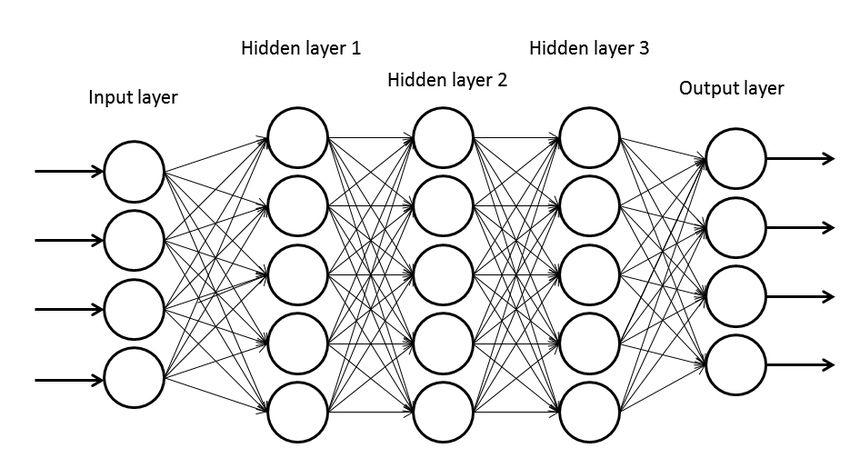
\includegraphics[width=140mm]{../img/dnn.png}
	\caption{An example of sequentially stacked fully connected layers. This architecture has three hidden layers. The number of neurons in all the layers can vary. Adapted from \citep{miralles2017methodology}.}
	\label{img01:dnn}
\end{figure}


Common activation functions used in artificial neural networks are the following:



\begin{enumerate}
	\item \textbf{Sigmoid}: The most basic activation function is the sigmoid function. Its application is common in binary classification as the sigmoid returns values between 0 and 1, which can be interpreted as probability of a certain class. It is, however, not used in hidden layers of deep neural networks as multiple sequentially stacked sigmoid functions cause an infamous \emph{vanishing gradient problem}, preventing the DNNs from learning effectively \citep{Goodfellow-et-al-2016}:
	\begin{equation}
		\sigma (x) = \frac{1}{1 - e^{-x}}
	\end{equation}
	\item \textbf{Tanh}: Another popular activation function tanh is based on sigmoid:
	\begin{equation}
		\tanh (x) = 2 \sigma(2x) - 1
	\end{equation}
	\item \textbf{Rectified Linear Unit (ReLU)}: ReLU is beneficial for tasks where an activation function has to return positive value. It is, therefore, an appropriate choice as the last activation of the DNNs for neural encoding prediction since the final value has to be non-negative. It is, however, also used in cases where positivity is not required:
	\begin{equation}
	\text{ReLU} (x) = \max(0, x)
	\end{equation}
	\item \textbf{Exponential Linear Unit (ELU)}: When $x \geq 0$, ELU acts as an identity. However, compared to ReLU, ELU can return negative values. ELU is known to perform well and improve DNN training. \citep{clevert2015fast}:
	\begin{equation}
	\text{ELU} (x) = \left\{\begin{array}{lr}
	\alpha (\exp(x) - 1), & \text{for } x \leq 0 \\
	x, & \text{for } x > 0 \\
	\end{array}\right\}
	\end{equation}
	\item \textbf{AdaptiveELU}: In prediction of neural population responses, non-negativity is appropriate due to the neural responses being positive. AdaptiveELU is a non-negative activation function that has the beneficial training properties of ELU. This is achieved by shifting ELU by a predefined offset.
	\begin{equation}
	\text{AdaptiveELU}(x) = \text{ELU}(x - x_{shift}) + y_{shift}
	\end{equation}
	\item \textbf{Softplus}: This activation function can be interpreted as a smooth ReLU.
	\begin{equation}
	\text{Softplus} (x) = \log(1 + \exp(x))
	\end{equation}
\end{enumerate}


\section{Training of the DNNs}

The objective of the DNN training is to find weights that minimize a chosen loss function $L(D, w)$. Due to the vast number of parameters, an enormous volume of data, and the nonlinear nature of DNNs, direct analytical solutions are not feasible. Instead, neural networks utilize gradient-based methods.

Very simply put, gradient methods minimize an objective function iteratively. Let $L(D, w)$ be a loss function that we wish to minimize. The basic gradient-based algorithm looks similar to this pseudocode:


\begin{algorithm}[H]
\begin{algorithmic}
	\caption{A gradient-based algorithm for finding the optimal weights $w$}\label{alg:grad}
	\State Randomly initialize $w$
	\While{$L(D, w)$ has not converged yet}
		\State $w \gets w - \alpha \nabla_w L(D, w)$
	\EndWhile
\end{algorithmic}
\end{algorithm}

As regards the weight initialization in the gradient-based algorithm (Algorithm~\ref{alg:grad}), more sophisticated initialization techniques yielding better results also exist \citep{glorot2010understanding}.

Intuitively, the model’s parameters are updated in a direction that should minimize the loss. How large steps we perform depends on the $\alpha$ hyperparameter called the learning rate, which can even change in every iteration (it usually decreases).

The crucial part is the computation of
\begin{equation}
	\nabla_w L(D, w) = \mathbb{E}_{(\textbf{x}, y) \sim \hat{P}_{data}} [ \nabla_w L((\textbf{x}, y), w) ].
\end{equation}

Although the gradient can be computed directly using the whole training dataset, this is not usually done due to the large data volume. A popular stochastic gradient descent algorithm (SGD) \citep{kiefer1952stochastic} randomly selects a subsample of the training dataset called a batch; let us denote it $B$ of $m$ samples. Then it estimates the gradient as follows:

\begin{equation}
	\hat{\nabla}_w L(D, w) = \frac{1}{m} \sum_{i=1}^m \nabla_w L((\textbf{x}, y), w).
\end{equation}
 

The SGD algorithm iteratively uses all batches in the dataset to update the weights, performing one so-called epoch of the training algorithm. Epochs are repeated until the $L(D, w)$ has not converged or we run out of time or patience.

Many other algorithms build upon the stochastic gradient descent. Specifically, a popular SGD variant, which has empirically proven to perform better, is a widely used algorithm Adam \citep{kingma2014adam}. In each step, this algorithm adapts the learning rate and a gradient’s direction. As a consequence, Adam tends to converge quicker than SGD.

\section{Regularization for Deep Neural Networks}

Besides $L_1$ and $L_2$ regularizations described in a general section about regularization, other techniques are also implemented for DNNs. The integral approach relevant to this thesis is batch normalization \citep{ioffe2015batch}, which adaptively normalizes the output of a certain layer to have a mean equal to 0 and unit variance in every batch, stabilizing and accelerating the training. We should also mention dropout \citep{srivastava2014dropout}, which sets during training a random portion of the input to the next layer to zeros. This prevents the network from having neurons specialized for specific training examples, helping to develop a robust network.

\section{Convolutional Neural Networks}

Despite the network composed of fully connected layers being a universal approximator, when applied to an image input, it has many parameters due to the vast number of pixels. In order to decrease the dimensionality of the parameter space and take advantage of the spatial or temporal properties of the data, a new architecture has been developed; a convolutional neural network (CNN).

This sequential architecture consists of stacked convolutional layers. Each layer has a three-dimensional input of dimensions $(H, W, C)$, where $H$ and $W$ stand for the input’s height and width, and $C$ stands for the number of channels. For example, a grayscale image has just one channel, and an RGB image has channels for red, green, and blue colors; hence $C = 3$. An RGB picture with a resolution of $1080 \times 1920$ would be of size $1080 \times 1920 \times 3$. In the forward pass of the input through the network, the dimensions of the features can change in every layer. 

The most prominent characteristic of the CNNs for visual input that distinguish them from other types of networks is their use of spatial properties. The prime focus is on the interactions of pixels in a local neighborhood, as their properties correlate more significantly than the properties of distant pixels. Trainable convolutional filters called kernels are thus used to capture relationships in rather small areas. They perform a linear operation called convolution.

\begin{defn}[Convolution]\label{def01:7}
	Let $I$ be a 3-dimensional input tensor of size $h \times w \times c$ and $K$ be a kernel of size $m \times n \times o$. Convolution of a tensor $I$ with a kernel $K$ is an operation defined as:
	\begin{equation}
		(K \star I)_{i, j, o} = \sum_{m, n, c} I_{i+m, j+n, c} K_{m, n, c, o}
	\end{equation}
\end{defn}

For a better understanding, we append a visual explanation of the convolution of an RGB image with two kernels (Figure~\ref{img02:conv}).

\begin{figure}[h]\centering
	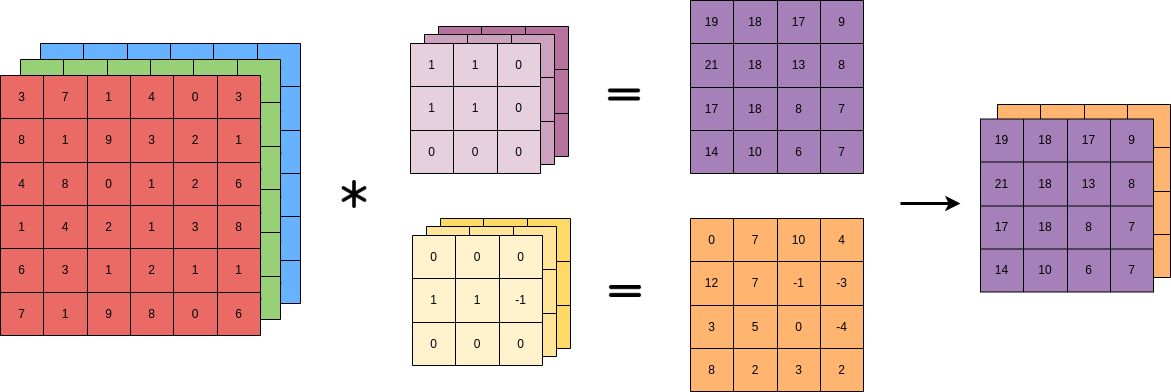
\includegraphics[width=140mm]{../img/convolution.png}
	\caption{A visualization of convolution operation of $6\times6\times6$ input. Two kernels are applied on every possible pixel creating an output of shape $4\times4\times2$.}
	\label{img02:conv}
\end{figure}

A convolutional kernel is applied in every possible position (kernel must lay inside the input tensor). Because the weights are the same during the “movement” along the input, they capture local features of the same type in every position. This reduces the number of parameters as the same properties do not have to be learned separately in different locations (the weights are shared), and, consequently, it leads to translation-equivariance, also called shift-equivariance.


\begin{defn}[Equivariance]\label{def01:8}
	Let $f$ and $g$ be functions of $M \to M$. A function $f$ is equivariant to a function $g$ if $f(g(x)) = g(f(x))$ for every $x \in M$.
\end{defn}

When applied to convolution neural networks, this definition means that a CNN receiving a shifted image as input returns features transformed by the exact translation in the feature map.

In computer vision, relevant features in images often do not depend on their exact position. Because CNNs compute complex features of an input image in a position-independent way, they are the perfect choice of architecture for tasks in this field. It is thus no wonder that CNN-based architectures outperformed numerous state-of-the-art computer vision solutions of the pre-neural-network era. Their application in neuroscience is also abundant as features learned by CNNs are shown to be surprisingly similar to those in cells of the primary visual cortex \citep{kriegeskorte2015deep}. This fact, along with an unarguably good performance on tasks in neuroscience \citep{cadena2019deep}, \citep{klindt2017neural}, makes CNNs a faithful functional model of the early visual pathway and consequently an adequate mathematical model for neural response prediction in the visual system.

\section{Rotation-Equivariant CNN (reCNN)}


The foremost feature of regular CNNs is their shift equivariance property. However, a typical image transformation to which CNNs with no adjustment are vulnerable is rotation. In order to have a potent network for computer vision, it can be beneficial to have CNNs with rotation-equivariance property in addition to translation-equivariance.

For this purpose, there exist group convolutions, a class of convolutions that generalize convolutional networks to larger groups of symmetries, the rotation being among them \citep{cohen2016group}. In group convolutions, the group operation is the transformation, in our case, rotation and group elements are all possible input transformations. Let us assume that we want our network to be equivariant to four orientations. Given an input image, the group elements are all its four rotations, and the group operation is a rotation by 90 degrees counter-clockwise. A graphical illustration of a group is usually used as in the following figure (Figure~\ref{img03:group}).

\begin{figure}[h]\centering
	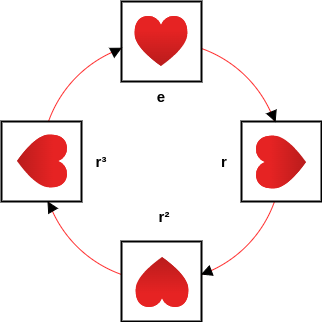
\includegraphics[width=80mm]{../img/group.png}
	\caption{A group of 4 rotations by 90\,degrees counter-clockwise. Elements are all four possible rotations depicted by a rotated heart. Arrows stand for one application of a transformation, in our case, rotation.}
	\label{img03:group}
\end{figure}

Firstly, a rotation-equivariant CNN creates every possible group element of the input. In our case, reCNN rotates each filter in the first layer to all allowed orientations and then applies a regular convolution with the input image. We do not rotate the input as the input is usually much larger than the filter. If we want to have 8~channels in the first layer, we obtain $4\times8 = 32$ new feature maps, each generated by one of eight kernels in one specific orientation.

This way, we have obtained a so-called structured feature map; features structured in groups, one for every rotation. In the subsequent layers, the computations are different. To compute one new output channel (for all rotations), a different filter is learned for every feature map from the previous layer, sticking to the assumed values, 8~filters have to be trained for every orientation. These kernels are applied to the input features, then rotated and cyclically permuted to the next group position. In this position, they are applied again, followed by another rotation and cyclic permutation. This is done for every orientation, in our case 4~times. At each element of the group, the convoluted feature maps are summed in a pointwise manner, creating an output feature for the given orientation. If we wanted to obtain more output channels, the same process would be performed with more sets of filters. Desiring 8~output channels, we would end up with $4\times8\times8 = 256$~filters. A visual explanation is appended in the following figure (Figure~\ref{img04:recnn}).

\begin{figure}[h]\centering
	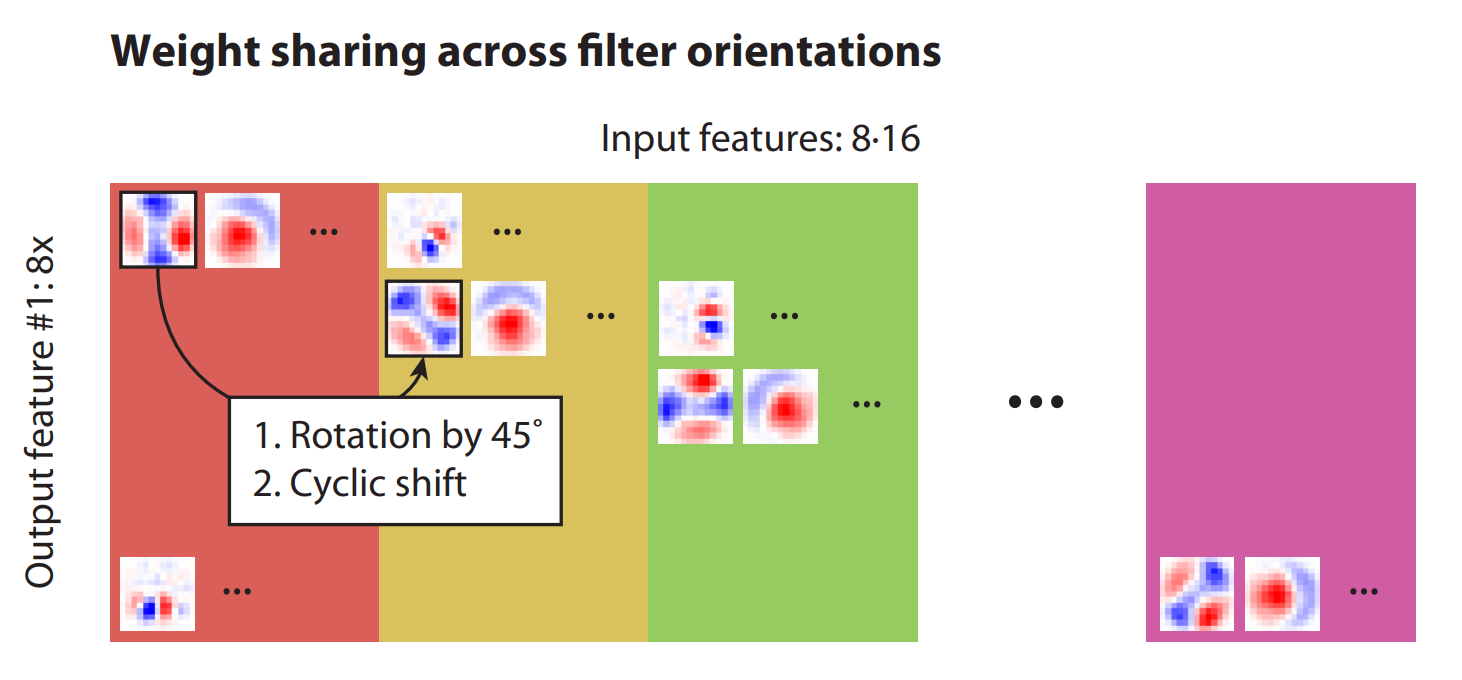
\includegraphics[width=140mm]{../img/reCNN_visualization.png}
	\caption{Illustration adapted from the work of Ecker et al. \citep{ecker2018rotation} uses 8~rotations and 16~channels. Every colored rectangle stands for filters from which new features of one given orientation are to be created, therefore, one color stands for one orientation. The filters are rotated by 45~degrees and cyclically shifted to compute the next orientation. On the vertical dimension, the number of kernels corresponds to the number of channels on output. The horizontal dimension has size~8; one filter for every orientation of the input.}
	\label{img04:recnn}
\end{figure}


Obviously, only four orientations of a square filter are achievable without interpolation artifacts. However, as we want to have an arbitrary number of orientations, this approach is insufficient. For this reason, a steerable basis of two-dimensional functions is employed as a filter representation. In this technique, which was proposed by Weiler et al. \citep{weiler2018learning}, the filter learns weights for the basis functions. As the basis is steerable, we can rotate the filter into any required orientation without interpolation artifacts.

\section{Evaluation metrics}

Although Poisson loss function is suitable for training of a machine learning model, it is not an ideal evaluation metric, as it depends on the scale and shift of the neural responses \citep{willeke2022sensorium}. This might complicate the comparison of models trained on different datasets.

\subsection{Averaged Pearson’s correlation}


Instead, we will measure Pearson’s correlation coefficient per neuron between the predicted and measured responses. The averaged Pearson’s correlation coefficient over all neurons will be used as the model’s performance metric. Additionally, the test set contains repeated measurements of neural responses to the same visual stimulus. We will average these responses and compute the correlation of our prediction to the average response, which will partially eliminate the neural response variability.

\begin{defn}[Pearson’s correlation coefficient]\label{def01:9}
	Given random variables $X$ and $Y$, the Pearson's correlation coefficient is defined as
	\begin{equation}
		\rho_{X, Y} = \frac{\mathbb{E}\left[(X - \mu_X)(Y - \mu_Y)\right]}{\sigma_X \sigma_Y},
	\end{equation}
	where $\mu_X$ and $\mu_Y$ are the means of the random variables X and Y, $\sigma_X$ and $\sigma_Y$ are the standard deviations of the random variables X and Y.
\end{defn}


In comparison to Poisson loss, Pearson’s correlation coefficient is a number from interval $[-1, 1]$, making this metric easier to interpret and thus more appropriate as an evaluation metric.

\subsection{Oracle Correlation and Fraction of Oracle}

In the chapter introducing the early visual system, we described the connections between V1 and other brain regions. The primary visual cortex is not solely dependent on the visual input. A substantial portion of input information comes from different brain areas. This is one of the reasons why neurons exhibit a significant response variability given the same visual stimulus.

We can consider this variability which cannot be explained merely by input features, in our case visual input, as a noise generated by unknown noise generating distribution. This distribution is responsible for the irreducible error defined in the Section~\ref{section:regression} about regression. We have laid a strong emphasis on this topic since, compared to datasets that the reader might have encountered in machine learning, the influence of noise is much more significant in neuroscientific datasets. Moreover, it is crucial to remember that different datasets contain different irreducible errors. Although independent of the scale of neural responses, correlation is not ideal as an evaluation metric as one model can achieve different correlations on distinct datasets.

To take into account the variability neurons exhibit, Walker et al. \citep{walker2019inception} have developed a metric called oracle correlation and fraction of oracle. For this purpose, the test set contains multiple trials with the same input image, enabling us to observe how the neural response varies. Firstly, we compute an oracle, an estimate of a maximal achievable correlation per neuron. It is done by computing the correlation of the leave-one-out mean and the remaining response from the repeated inputs. We then average the correlation over all neurons.

Finally, the fraction of oracle achieved by the model is estimated as a slope of a linear function without offset fitted on oracle correlation to the model's test set correlation across all neurons.

This technique guarantees a better performance estimation given a dataset where noise significantly influences the target values. It can also be used to compare models trained on different datasets, as it is independent of the intrinsic noise. However, there are drawbacks, too. Firstly, it is necessary for the test set to consist of repeated trials. Secondly, the performance estimation is influenced by the number of repeats. If the number of repeats is low, the estimate of oracle fraction performance can return a value higher than 1.


\section{Ensemble learning}

Ensemble learning is a machine learning technique based on the idea that a combination of multiple different hypotheses might lead to a hypothesis with a better predictive performance. This approach is usually utilized when the hypotheses are very different. However, deep learning ensemble models containing the same model architecture with different random weight initialization often achieve higher performance than just one standalone model of the same type \citep{fort2019deep}.

Although the rules for combining the models can be complex, even fairly simple rules can be effective. In the regression task, an average of each model’s prediction is often used as the prediction of the whole ensemble model.












